\documentclass{article}

\usepackage{graphicx}

\newcounter{exo}

\newenvironment{exercise}%
{\par\vspace{.5\baselineskip}\noindent
\refstepcounter{exo}%
\textbf{Exercise \theexo}%
\par\vspace{.5\baselineskip}\noindent\ignorespaces
\begin{center}\begin{minipage}{0.9\linewidth}}%
{\end{minipage}\end{center}\smallskip}

\usepackage{paralist}
\usepackage[margin=2.5cm]{geometry}

\begin{document}
\pagestyle{empty}

\begin{center}
\Large Scientific Software Development in Python, AIMS Rwanda 2016 \\ \smallskip
Assignment week 1
\end{center}

For this first assignment you are asked to create a Jupyter notebook in which
you will solve the exercises. Normally you have also downloaded a notebook
template to start from.

Each function should come with
\begin{compactitem}
\item some examples
\item some tests that check that the result is consistent. For example if you have
programed the \texttt{gcd} function you can have the following in the cell after
\begin{verbatim}
# the code below checks the consistency of the gcd function
for a in range(50):
    for b in range(50)
        assert gcd(a, b) == gcd(b, a)
        assert gcd(a + b, b) == gcd(a, b)
        for c in range(10):
            assert gcd(c*a, c*b) == c * gcd(a, b)
\end{verbatim}
\end{compactitem}

\noindent A lot of attention will be paid to the clarity of the code. In particular
\begin{compactitem}
\item The corrector should be able to run your cells from top to bottom
without getting any error (you can try the command "Kernel $\to$ Restart and Run All"
from the Jupyter menu).
\item Do not put to many instruction inside a given cell. For example,
no more than one function.
\item give meaningful names to your variables, for example \texttt{s} for a
sum and \texttt{p} for a product, \texttt{counter} for a counter in
a \texttt{range}, etc
\item use comments (using \texttt{\#}) to explain the delicate steps
of your algorithms
\end{compactitem}


\begin{exercise}
A Pythagorean triplet is a set of three positive numbers, $x < y < z$, for which,
$x^2 + y^2 = z^2$. For example, $3^2 + 4^2 = 9 + 16 = 25 = 5^2$. There exists
exactly one Pythagorean triplet for which $x + y + z = 1000$. Find this triplet.
\end{exercise}

\begin{exercise}
Write a function \texttt{prod(l)} that returns the product of the elements in
the list \texttt{l}. In case the list is empty, the function should return
\texttt{1}.

\smallskip\noindent
For example
\begin{verbatim}
>>> prod([1, 3, 2, 3])
18
>>> prod([])
1
\end{verbatim}
\end{exercise}

\begin{exercise}
Write a function \texttt{gcd(x, y)} that computes the greatest common divisor
of two integers using Euclide algorithm.

\smallskip\noindent
Plot the graphic of the function $n \mapsto \# \{(p,q): 1 \leq p \leq n,\ 1 \leq q \leq n,\ \gcd(p, q) = 1\}$.

\smallskip\noindent
Could you guess the asymptotic?
\end{exercise}

\newpage

Recall that the \emph{digits} of an integer $n$ in base $b$ is the sequence of numbers $(n_0, n_1, \ldots, n_d)$
in $\{0, 1, \ldots, b-1\}$ so that
\[
n = \sum_{i=0}^d n_i b^i.
\]
For example, the digits of $12$ in base 10 are $(2,1)$ and in base $2$ are $(0,1,1)$.
\begin{exercise}
Write a function \texttt{digits(n, b)} that return the list of digits of the number \texttt{n} in base \texttt{b}.

\smallskip\noindent
Let $n = 123576537645123412$ written in base 10. What are its digits in base 2? In base 3?

\smallskip\noindent
What is the sum of the digits of $2^{100}$ written in base 3?
\end{exercise}

\begin{exercise}
Using \texttt{plot} from \texttt{matplotlib.pyplot}, build this sequence of figures
\begin{center}
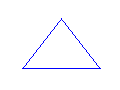
\includegraphics{triangle0.pdf} 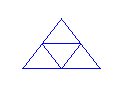
\includegraphics{triangle1.pdf} 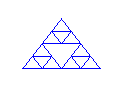
\includegraphics{triangle2.pdf} 
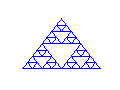
\includegraphics{triangle3.pdf} 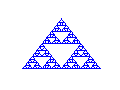
\includegraphics{triangle4.pdf}
\end{center}
For that purpose, you might want to use a recursive function of the form
\begin{center}
\texttt{triangle(x0, y0, x1, y1, x2, y2, n)}
\end{center}
that draws a triangle with vertices $(x_0, y_0), (x_1, y_1), (x_2, y_2)$ and if $n > 0$ calls
itself with appropriate new coordinates and $n-1$.
(see worksheet 3).
\end{exercise}

\end{document}
